\documentclass[preprint]{sigplanconf}
\usepackage{xspace,url,subfigure,,framed,
            hyperref, graphicx, fancyvrb % double brackets llbracket
}

\usepackage[T1]{fontenc}
\usepackage{beramono}
\usepackage{listings}
\usepackage{textcomp}
\usepackage[usenames,dvipsnames]{xcolor}
\usepackage{amsmath}

\lstdefinelanguage{Julia}%
  {morekeywords={abstract,break,case,catch,const,continue,do,else,elseif,%
      end,export,false,for,function,immutable,import,importall,if,in,%
      macro,module,otherwise,quote,return,switch,true,try,type,typealias,%
      using,while},%
   sensitive=true,%
   morecomment=[l]\#,%
   morecomment=[n]{\#=}{=\#},%
   morestring=[s]{"}{"},%
   morestring=[m]{'}{'},%
}[keywords,comments,strings]%

\lstset{%\lstinputlisting[language=Octave]{BitXorMatrix.m}
    language         = Julia,
    basicstyle       = \small\ttfamily,
    keywordstyle     = \bfseries\color{blue},
    stringstyle      = \color{magenta},
    commentstyle     = \color{ForestGreen},
    showstringspaces = false,
    stepnumber=1,
    numbers=left
}

\newcommand{\rn}[1]{#1}
\newcommand{\doi}[1]{doi:~\href{http://dx.doi.org/#1}{\Hurl{#1}}}

\newcommand{\xt}[1]{\texttt{#1}}

\newcommand{\OK}[1]{#1\;\text{OK}}
\newcommand{\abstype}[2]{\xt{abstract}~#1 <: #2}
\newcommand{\oftype}[2]{#1::#2}
\newcommand{\m}[2]{{#1}(#2)}
\newcommand{\contype}[2]{\xt{type}~#1 <: #2}	
\newcommand{\any}{\xt{any}}
\newcommand{\jolt}{\xt{Jolt}}

\newcommand{\exact}[1]{{\llbracket #1 \rrbracket_{\xt{exact}}}}
\newcommand{\usable}[1]{{\llbracket #1 \rrbracket_{\xt{}}}}
\renewcommand{\ldots}{...}
\newcommand{\cnum}[2]{$\text{#1}_#2$}

\usepackage{stmaryrd}
\usepackage{amssymb}
\usepackage{mathpartir}

\conferenceinfo{NOOL '16}{Month d--d, 20yy, City, ST, Country} 
\copyrightyear{20yy}
\copyrightdata{978-1-nnnn-nnnn-n/yy/mm}
\copyrightdoi{nnnnnnn.nnnnnnn}
\begin{document}
\title{Bottom-up Objects --- Static Typing Without Types} 
\authorinfo{Benjamin Chung \and Paley Li \and Jan Vitek}{Northeastern University}{bchung@ccs.neu.edu \and \{pa.li,j.vitek\}@neu.edu} % Annon : Benjamin Chung, Jan Vitek}{Northeastern University}{}
\maketitle
% We should probably have some more introductory/motivational material herezies

\begin{abstract}
Julia is an untyped imperative programming language designed for scientific computing. 
Despite being untyped, however, Julia provides a rich runtime type systems that includes features such as  
inheritance. As the language has no mechanism to enforce functional interfaces, Julia programs 
are subjective to improper assumptions about an untyped interface. We propose a static type system for a 
subset of Julia, called \jolt, that rules out functional interface mismatches
with no syntactic alteration to the core of Julia.
\end{abstract}


\section{Introduction}

Traditional statically typed object-oriented languages have a series of
common idioms: single dispatch~\cite{jls}, figuring out which method
to use in which situation, interfaces~\cite{objinter, fj}, abstracting over 
common means of access, and the means to statically
ensure that those interfaces are adhered to with the correct dispatch call.

These practices are perfectly suitable for many contexts,
as is demonstrated by the success of Java~\cite{jls}, C\#~\cite{csls}, and C++~\cite{cppls}, 
These features are not universally applicable, however, some languages that do not have these features
can still use object abstraction to retain static safety[\textcolor{red}{cite}].

Julia is one such programming language, as it provides multi-method dispatch 
and an interface system that focuses on an abstract struct-like construct. 
Julia was originally designed for the purpose of scientific compution, in the vein of 
R [\textcolor{red}{cite}]or Matlab[\textcolor{red}{cite}], as such contains a number of features designed specifically to support 
numeric computation and other tasks common in scientific programs.

\begin{figure}[h]

\lstinputlisting[language=Julia]{broken.jl}
\begin{Verbatim}[fontsize=\small]
ERROR: MethodError: no method matching a(::C3)
Closest candidates are:
  a(::C1)
  a(::C2)
\end{Verbatim}
\caption{Object inheritance example in Julia.}
\label{code:broken}
\end{figure}


\begin{figure}
\centering
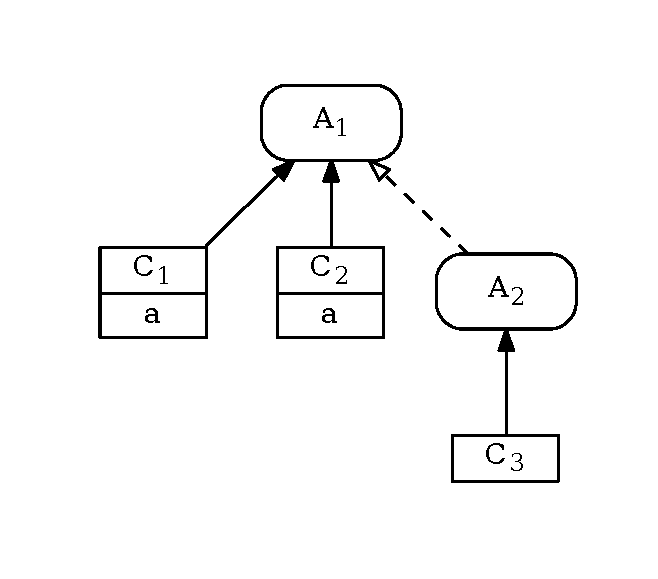
\includegraphics[scale=.6]{example2.pdf}
\caption{Inheritance hierarchy diagram for figure~\ref{code:broken}.}
\label{fig:algo}
\end{figure}

\section{Julia}

From the perspective of an object-oriented paradigm, Julia has several interesting features:
\begin{itemize}
\item Julia is \emph{dynamically typed}, and has no mechanism for statically
checking type correctness. However, as illustrated in figure~\ref{code:broken},
Julia code has many types.
\item The reason for all of these types is \emph{dispatch}. Julia provides 
full multi-method dispatch based on \emph{runtime type tags}, letting programmers
write code that is highly specified for a specific value.
\item Julia does not allow explicit procedural interfaces, a key feature of traditional 
object systems. Julia's interfaces are called \emph{abstract types}, and they 
define no explicit methods, instead, the abstract types rely upon ``a collection of informal interfaces''
\cite{juliadocu} to abstract over implementations.
\end{itemize}

Figure~\ref{code:broken} provides an illustration of how these features 
interact, and how they can be used to do untyped object-oriented programming.
The figure begins by constructing the object hierarchy shown in figure~
\ref{fig:algo}, then adds the method \xt{a} to the concrete classes $\text{C}_1$ and
$\text{C}_2$. The last function definition adds a function \xt{problem} to the
program, which calls the function \xt{a} on an argument of type $\text{A}_1$.

The next step is to actually call the methods we have defined. Julia performs
dispatch by looking for the \emph{most specific method} whose arguments are
satisfied by the given value - in essence, giving us a type guarantee that the
argument will always be of the declared type. In this way, the implementation 
of \xt{a} on line 7 is called when we call \xt{a} with an instance of $\text{C}_1$,
and the implementation of \xt{a} on line 8 is called for $\text{C}_2$.

However, the unchecked nature of Julia interfaces becomes apparent when we consider
$\text{A}_2$ and $\text{C}_3$. \cnum{C}{3} has no $\xt{a}$ implementation, and
therefore, despite being a subtype of \cnum{A}{1} 
(transitively, through \cnum{A}{2}), a call to \xt{a} with an instance of \cnum{C}{3}
fails with the error that no implementation of $\xt{a}$ exists for \cnum{C}{3}.

This problem is easy to spot in this example, because all of the type definitions
are simple and in the same place. However, in a real Julia program, types can be
imported from other files and exist in much larger hierarchies than the one seen
here. As a result, errors where a functional interface is violated by a library
are possible, and can be difficult to detect ahead of time.

Real Julia programs do have a lot of statically available information, however.
Julia programmers add a lot of types to their functions, associating the functions
with the types that they can work with. We can use this information to statically
built interfaces from the bottom up - taking the implementations and inferring the
interface that they all share.

\section{\jolt}
An interesting observation about the issue identified in figure~\ref{code:broken}
is that it can be seen as a ``message not understood'' error, exactly the kind
that type systems are widely applied to detect and prevent. However, untyped 
languages are uniquely difficult to type, as complex inference is typically
required and the idioms are difficult to track with types.

Despite being untyped, however, as mentioned previously Julia has a considerable
number of types, though they are not used statically. We propose a type system
for \emph{existing} Julia code that is able to statically detect the functional
interfaces that are implicit in Julia type hierarchies and method definitions,
and propose that this system can prevent ``method not found'' errors.

As Julia provides a complex and rich type system in conjunction with a moderately
complex syntax, we have constructed a heavily paired down version of Julia that we call \jolt.

\begin{figure}
\begin{align*}
t ::=~&  C ~|~ s\\
s ::=~& A ~|~ \any\\
d ::=~& \abstype{A}{s} ~|~ \contype{C}{s} \\
  & |~ \m{m}{\oftype{a}{t}, ~\ldots} = e\\
e ::=~& x ~|~ \xt{new} ~ C() ~|~ m(e,~\ldots) \\
\end{align*}
\caption{Static syntax for \jolt.}
\label{fm:syntax}
\end{figure}

\jolt\space formalises a minimal subset of Julia. In figure~\ref{fm:syntax}, we present the entire
syntax for \jolt, which consists of types (\xt{t}), declarations (\xt{d}), and expressions (\xt{e}). 
Types in \jolt\space are either a name, which can be the name of an abstract type (\xt{A}) or a concrete type (\xt{C}), 
or the \any\space keyword, which denotes the top type. The declarations 
of \jolt\space consists of declaring an abstract type, declaring a concrete type, and defining the body of a method.
The three expressions in \jolt\space are local variables, object creation, and method invocation. 

Due to the concise nature of this formalise, the expression typing and operational semantics rules for \jolt has
been omitted, as they are straightforward and does not offer much insight into the inheritance structure of Julia. 
Instead, we will focus our attention to highlight how \jolt\space generates and ensures correctness of the inheritance
hierarchy created from it's abstract and concrete types. 

\begin{figure}
\begin{mathpar}
\inferrule*[lab={\tiny TAbsSelf}]{ \m{m}{\ldots, \oftype{a}{A}, \ldots} \in \usable{A}}{ \m{m}{\ldots, \oftype{a}{A}, \ldots} \Subset A}

\inferrule*[lab={\tiny TConSelf}]{ \m{m}{\ldots, \oftype{a}{C}, \ldots} \in \usable{C}}{ \m{m}{\ldots, \oftype{a}{C}, \ldots} \Subset C}

\inferrule*[lab={\tiny TAbsChild}]{
	\forall\,C <: A: \m{m}{\ldots, \oftype{a}{C}, \ldots} \in \usable{C}\\ 
	\forall\,A' <: A: \m{m}{\ldots, \oftype{a}{A'}, \ldots} \Subset A'}
{ \m{m}{\ldots,\oftype{a}{A}, \ldots} \Subset A}

\end{mathpar}
\caption{Method enclosure over types.}
\label{fm:methInc}
\end{figure}

In figure~\ref{fm:methInc}, we present our rules for when methods are enclosed and/or inside a type.
The symbol $\in$ denotes the standard set notion for an element being inside a set. In \jolt,
this means the method is syntactically defined for the type it is in. The symbol $\Subset$ denotes a method being enclosed inside a type. 
In \jolt, a method is enclosed in a type if that method exists in the inheritance hierarchy, but there might not necessarly exist an actual implementation
of that method in the enclosing type. It is important to note the difference between $\Subset$ denoting the semantical relation of methods inside a type that represents it's place 
on the inheritance structure, while $\in$ denoting when a method is syntactically defined for a type.

The \textit{TAbsSelf} rule describes when an enclosing method is defined inside that type. 
For concrete types, their enclosing methods are always defined inside themselves, as reflected by the \textit{TConSelf} rule.
The \textit{TAbsChild} rule describes the case when an enclosing method in an abstract type 
is not inside that abstract type, which means it's concrete types must have this method inside them
and that all abstract types below this abstract must have this method enclosed within them.

To show an abstract type is correct requires to show three separate components. The first component shows the name of the abstract type is well-formed, 
the second component shows each method in the abstract type is well-formed, and the final component shows every method in the abstract 
type is enclosed within the abstract type. Similarly there are three parts for showing a concrete type is correct with respect to the definition
of concrete types.

The key to the implementation of this static type system is computing the 
enclosure relation to satisfy the requirements laid out in figure~\ref{fm:methInc}.
We propose the trivial approach, where the methods that are enclosed in some
abstract type $A$ are computed by taking the intersection of all abstract subtypes
$A'$ and concrete subtypes $C$, unioned with the methods that are defined for $A$
itself. 

\section{Conclusion}

Julia provides an interesting alternative to traditional functional interface 
definition, whereby the methods of an interface are solely defined by 
the concrete implementations of that interface, instead of having the interface specifying
the methods of it's concrete implementation. Despite being
untyped, we are able to utilize this property to create and reason statically about an inheritance
hierarchy within Julia. We demonstrate this approach in \jolt\space, a minimal subset
of Julia. \jolt\space provides static type checking for safe calls of multi-method.

The concept of patching against multi-method is not a novel or new technqiue, concepts such 
as Haskell's type classes and Rust's trait systems behaves similarly.

Our approach towards \jolt originated from the typed runtime of Julia, which has the potential to
provide the basis for other static analyses. New language features, such as purity, has the possibility
to be introduced in the future as types are already extensively used within Julia code.

\bibliographystyle{plain}
\bibliography{main}
\end{document}